
\section{Analoge Schaltung}
Im Kapitel werden die verschiedenen analogen Schaltungsteile näher erläutert. Dies entspricht der Messstrecke vom Shunt bis an den Mikrocontroller.
\subsection{Layer 1}%Marc 1 Seite
%%%%%%%%%%%%%%%%%%%%%%%%%%%%%%%%%%%%%%%%%%%%%%%%%%%%%%%%%%%%%%%%%%%%%%%%%%%
Der erste Layer ist für alle Schaltungsteile mit 230V, sowie für die Verbindung nach Aussen zuständig. Abbildung \ref{fig:first_layer} zeigt den groben Aufbau. Das genaue Schema befindet sich im Anhang unter \textbf{evt. Referenz hinzufügen!!!}

\begin{figure}[H]
\begin{center}
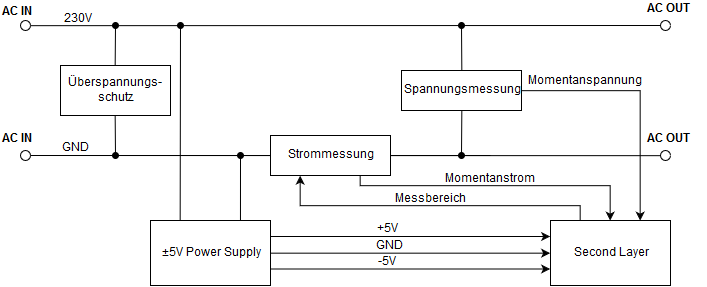
\includegraphics[width=160mm]{images/first_layer.png}

	\caption{Blockschaltbild des ersten Layers des Leistungsmessgerätes} %picture caption
	\label{fig:first_layer}
\end{center}
\end{figure}

\subsubsection*{Überspannungsschutz:}
Der Überspannungsschutz schützt das Gerät von Spannungen über 400V. Der Rest des Gerätes ist somit für bis 400V ausgelegt. Da das Gerät mit Wechselstrom betrieben wird, ist ein Verpolungsschutz unnötig. Einzig wird die Masse des Gerätes auf 230VAC schweben, falls das Gerät anders als geplant betrieben wird.

\subsubsection*{Strommessung:}
Für die Strommessung stehen zwei Messschunts zu Verfügung. Zum einen ein $50m\Omega$ Widerstand und zum anderen ein $1m\Omega$ Widerstand, welcher mit einem Relais parallel zum Ersten geschaltet werden kann. Durch die Parallelschaltung kann der Messbereich bei Betrieb umgeschaltet werden, ohne einen Unterbruch zu erzeugen, bei welchem, aufgrund induktiven Lasten, hohe Spannungen entstehen könnten, welche die Schaltung zerstören würden. Zudem kann somit eine unterbruchfreie Versorgung der Last gewährleistet werden. Für die Messung wird die Spannung vor dem Shunt bezüglich Masse (GND) gemessen.

\subsubsection*{Spannungsmessung:}
Die Spannung wird durch einen Spannungsteiler mit dem Verhältnis $\frac{7.5}{1000}$ gemessen, was bei einer Spannung von $\pm 400V$ zu einem Messsignal von $\pm 3V$ führt. Da der Messbereich des ADCs $\pm 2.5V$ beträgt, können maximal Spannungen von $\pm 333V$ gemessen werden.

\subsubsection*{Power Supply:}
Das Netzteil versorgt den gesamten Gleichstromteil der Schaltung. Es stellt einen maximalen Strom von $400mA$ zur Verfügung.

%%%%%%%%%%%%%%%%%%%%%%%%%%%%%%%%%%%%%%%%%%%%%%%%%%%%%%%%%%%%%%%%%%%%%%%%%%%
\subsection{Filter}

Wie schon im Kapitel technische Grundlagen werden die Filter gebraucht um harmonische Oberwellen herauszufiltern. Im Projektauftrag [x] wird definiert, dass Oberwellen ab 5kHz nicht mehr im Signal erwünscht sind. Darum müssen Oberwellen die eine höhere Frequenz haben, unterdrückt werden damit diesen nicht die Messung verfälschen.

\begin{minipage}[h]{0.5\textwidth} 
\begin{figure}[H]
\begin{center}
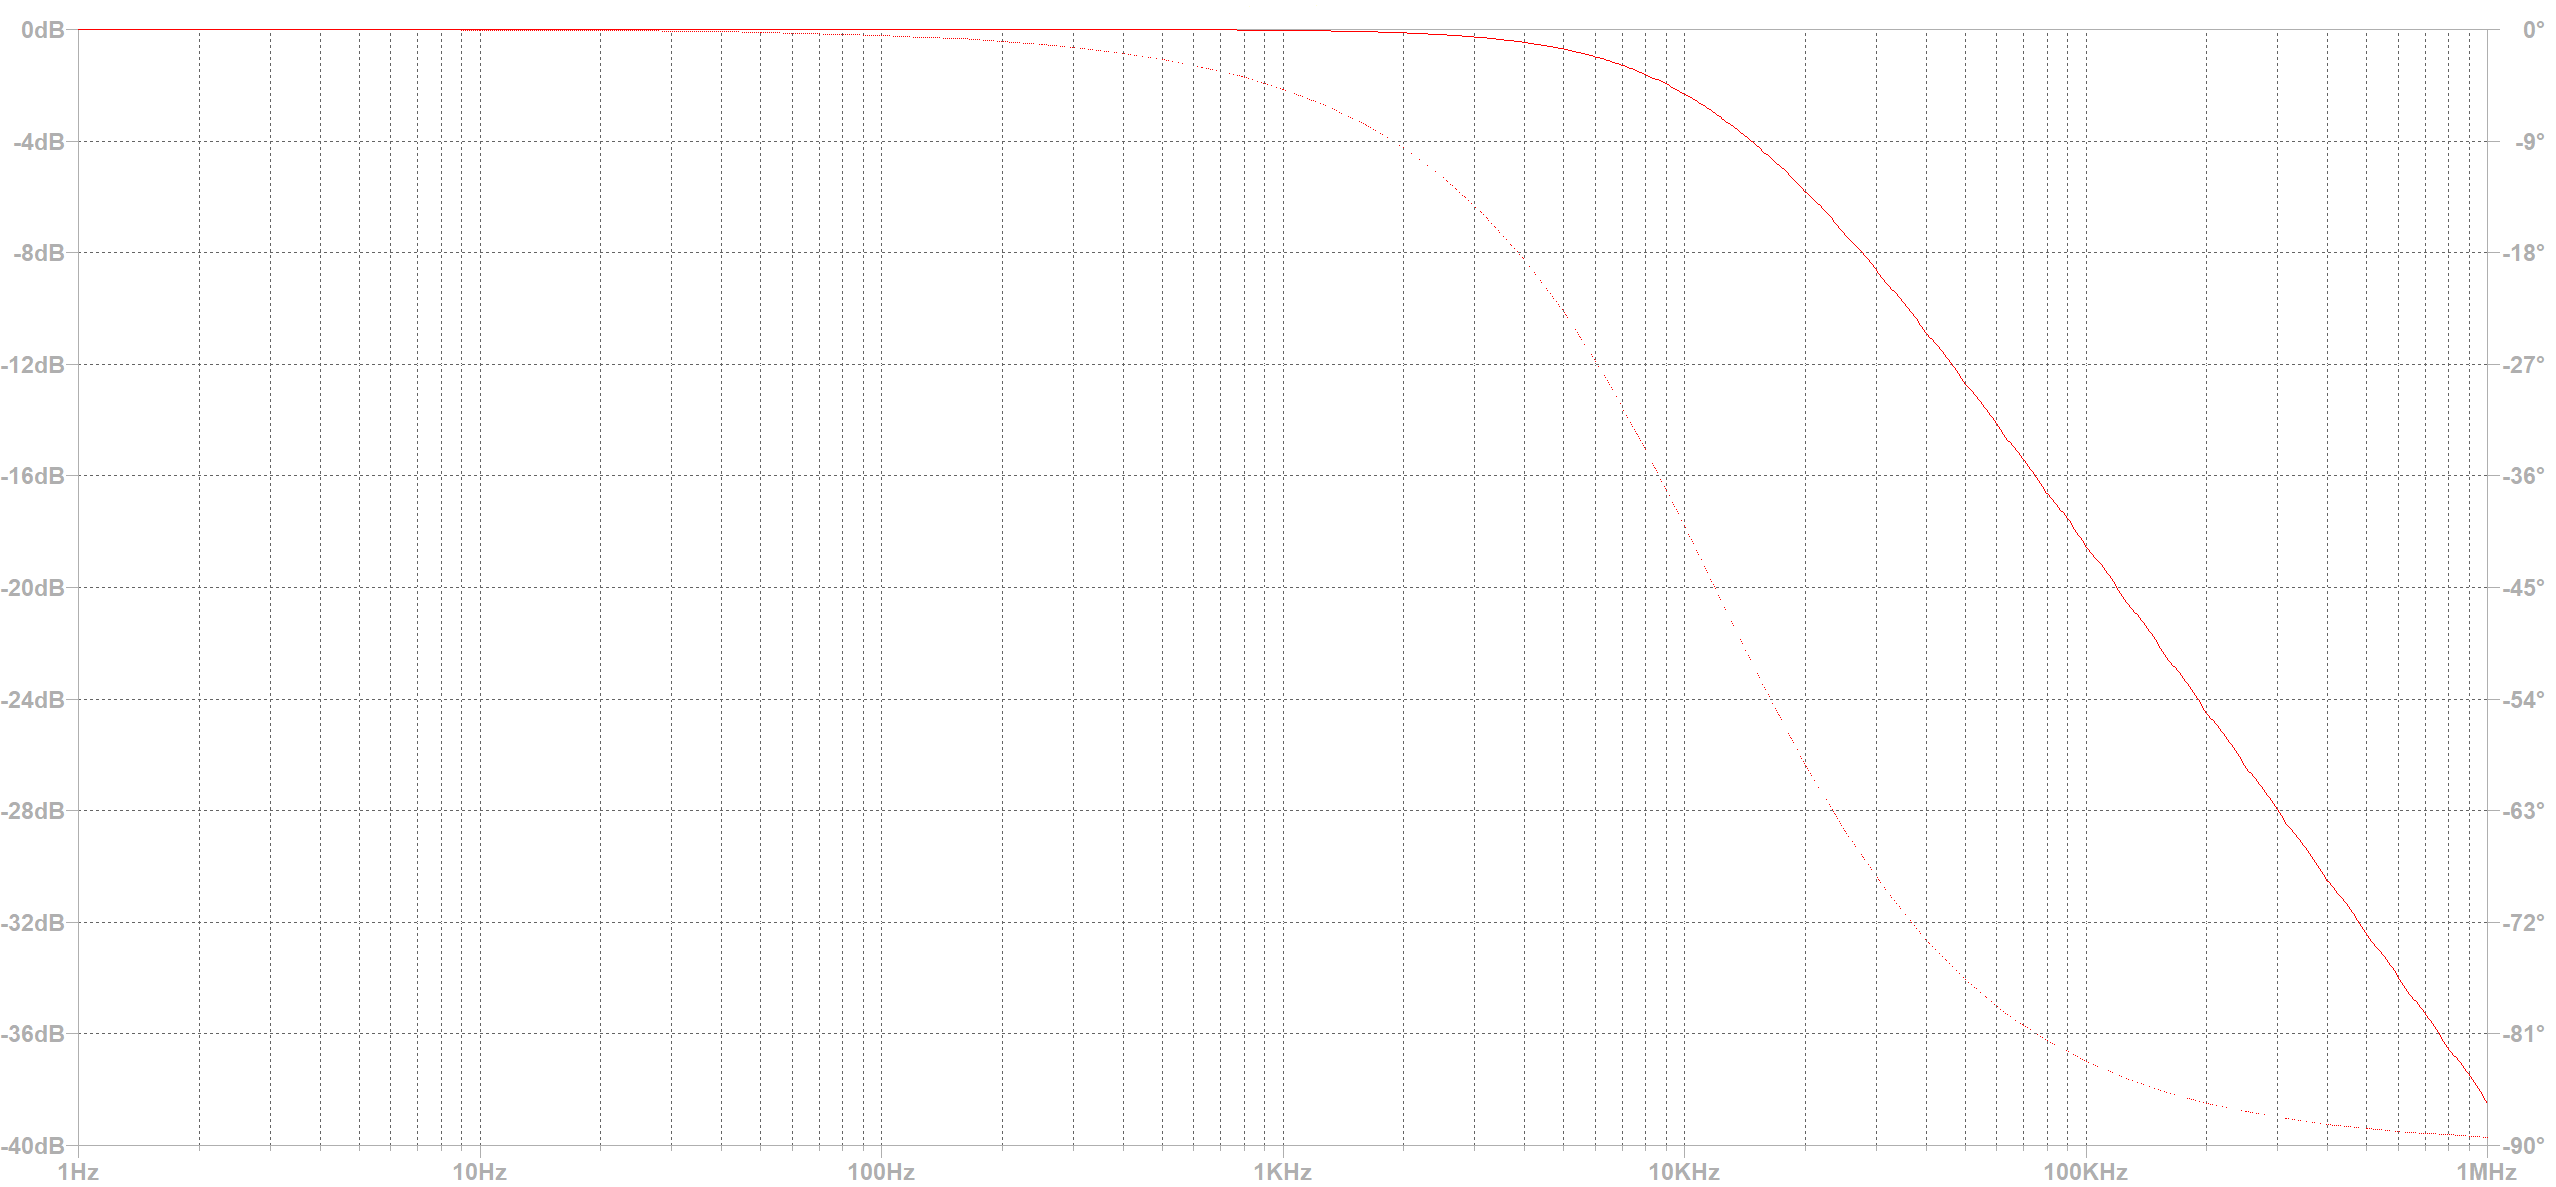
\includegraphics[width=0.9\textwidth]{images/Analoge_Schaltung_Frequenzgang.png}
\caption{Frequenzgang Tiefpass-Filter 1. Ordnung}
\end{center}
\end{figure}
\end{minipage}
\begin{minipage}[h]{0.5\textwidth}
Für das Projekt sind Tiefpass-Filter notwendig die höhere Frequenzen unterdrücken und tiefe Frequenzen passieren lassen. Auf dem nebenstehenden Bild ist ein typischer Frequenzgang eines Tiefpass-Filters 1. Ordnung zu sehen. Da für das Projekt die Signale auch verstärkt werden müssen, sind aktive Filter naheliegend.[x]
\end{minipage}


\subsubsection*{Dimensionierung}

\begin{minipage}[h]{0.5\textwidth}
Die Wahl fiel auf Butterworth-Filter mit Sallen/Key-Topologie 2. Ordnung. Diese bietet den Vorteil, dass sie nicht invertierend ist. Dadurch ist ein Operationsverstärker ausreichend pro Signalpfad. Die Butterworth-Koeffizienten bringen den Vorteil, dass sie flach sind im Durchlassbereich und einen relativ eckigen Übergang bieten.[x] Jedoch wurde überlesen, dass mit dieser Filtertopologie nur Verstärkungen bis $A=3$ realisierbar sind. Bei höheren Verstärkungen können die instabil werden. 
\end{minipage}
\begin{minipage}[h]{0.5\textwidth} 
\begin{figure}[H]
\begin{center}
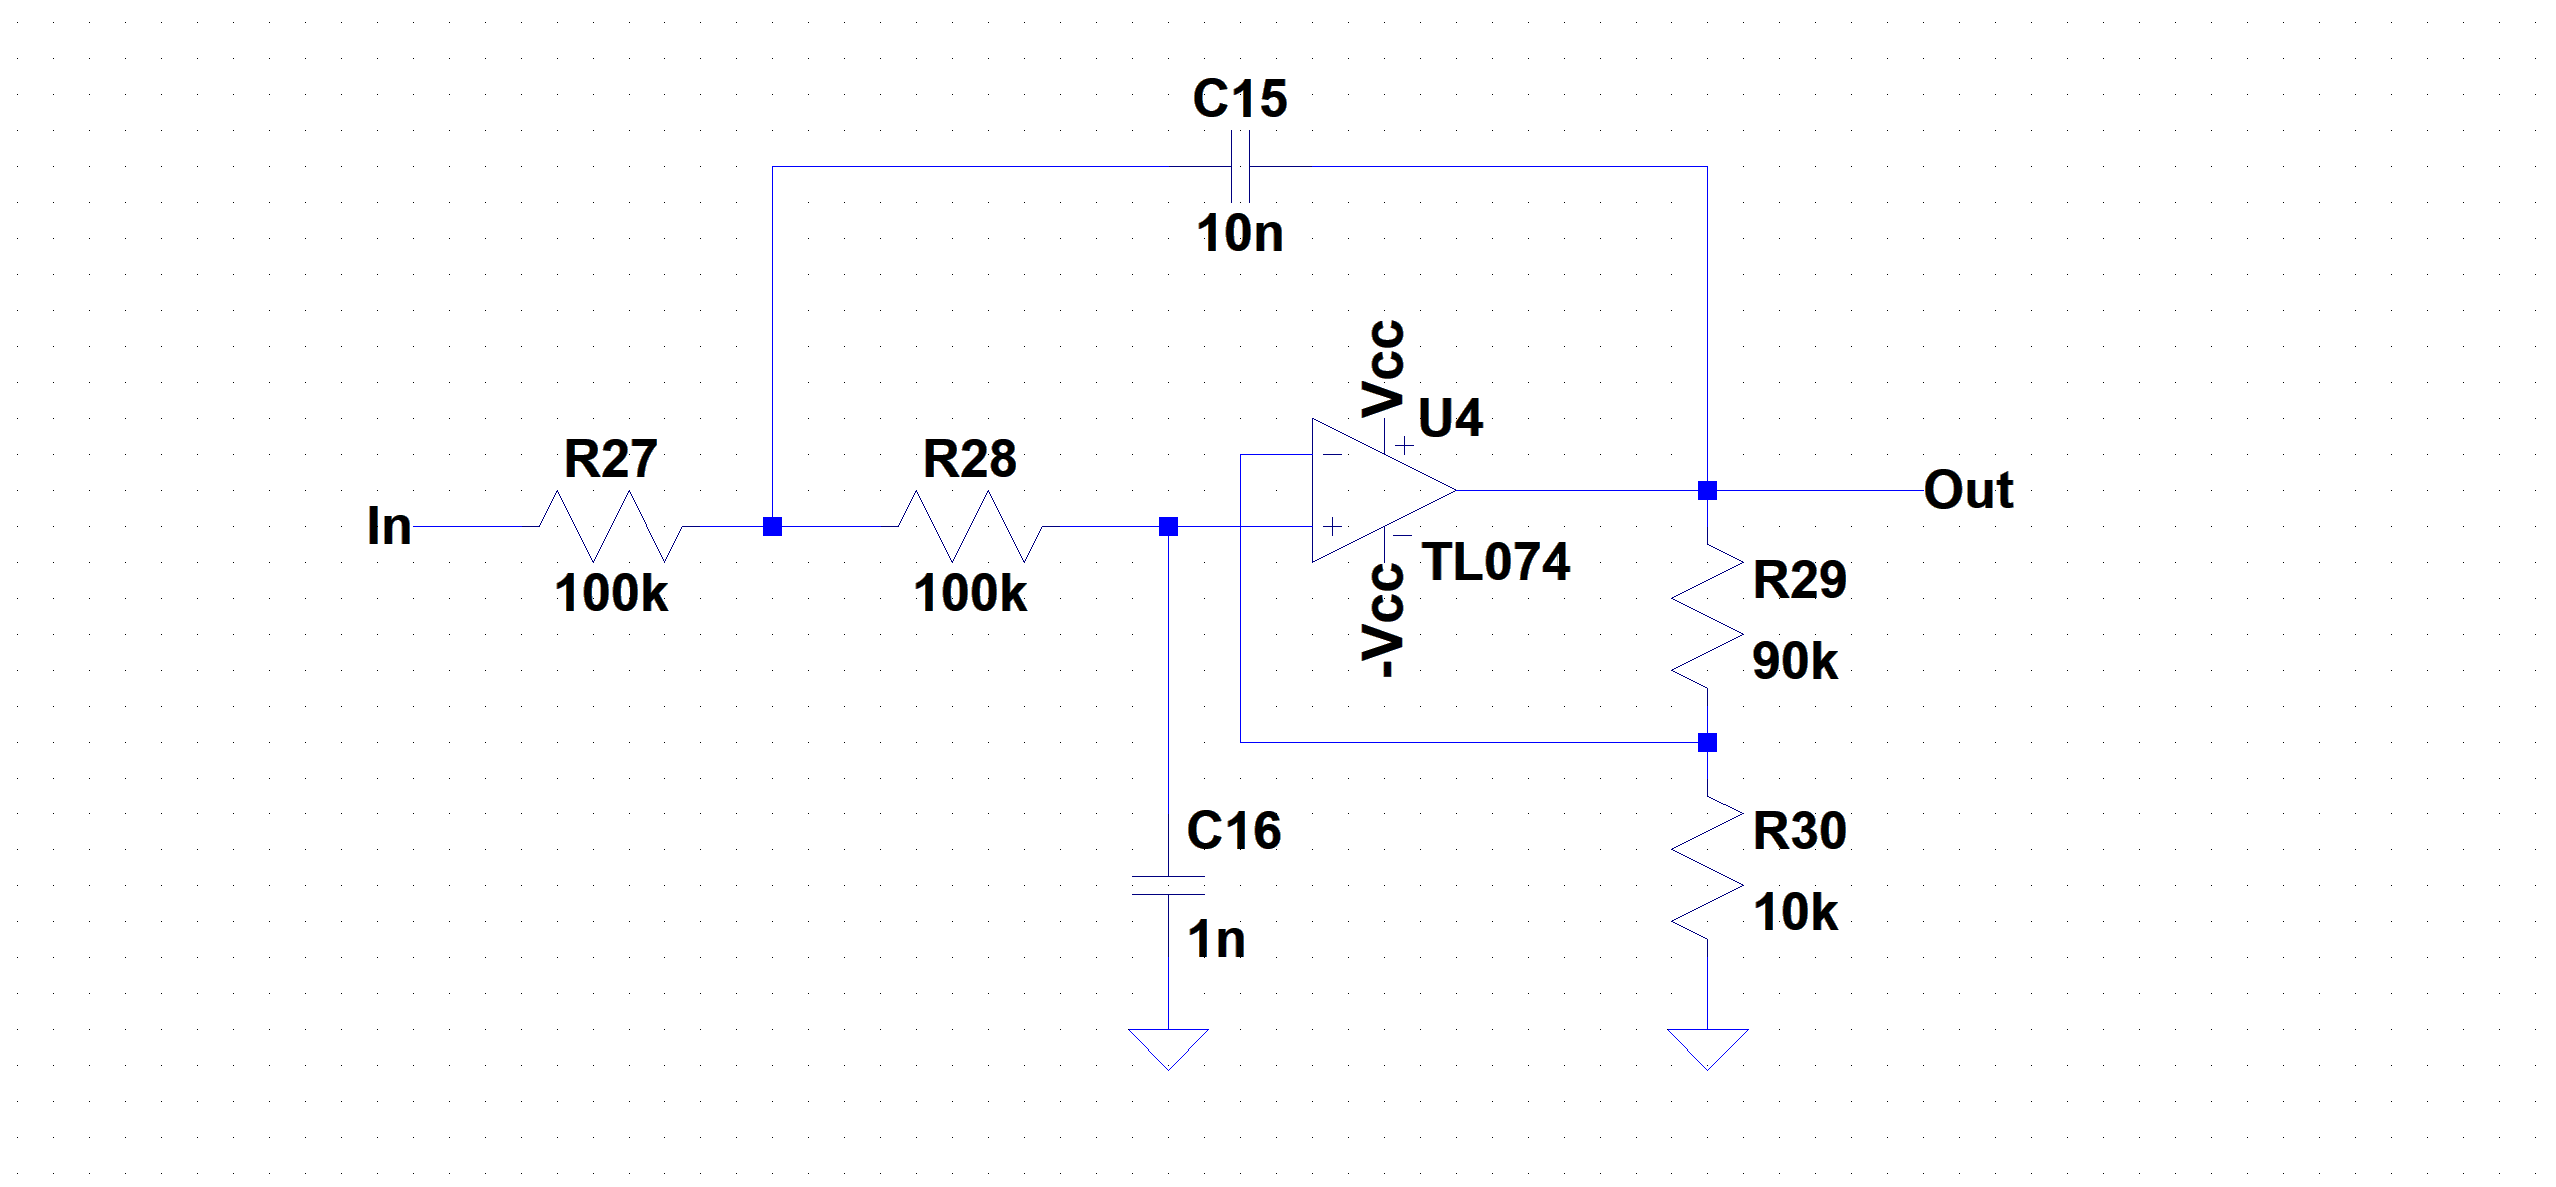
\includegraphics[width=0.9\textwidth]{images/Analoge_Schaltung_Sallen.png}
\caption{Sallen/Key-Topologie Tiefpass-Filter 2. Ordnung}
\end{center}
\end{figure}
\end{minipage}


\subsubsection*{Realisierte Filter}
Zuerst wurden die Sallen/Key-Filter realisiert. An den Operationsverstärker wurden praktisch keine Anforderungen gestellt. Er soll ein GWP[x] von mindestens 800kHz besitzen und nicht Rail-to-Rail sein. Dadurch wurde einer verwendet der an Lager war. Dies ist der TL074, der praktischerweise 4 Operationsverstärker in einem Gehäuse vereint. Die passiven Bauteile wurden mithilfe einer Formel[x] aus dem Internet erstellt, die sich im Laufe des Projektes als falsch herausstellte.

\begin{minipage}[h]{0.5\textwidth}
Nachdem der Print gefertigt war, wurde beim Testen festgestellt, dass die Filter instabil laufen aufgrund den zu hohen Verstärkungsfaktoren. Aus der Not wurden die Filter umgebaut in einen passiven Filter 1. Ordnung,gefolgt von einer Verstärkerschaltung. Dafür musste nur der Kondensator C15 entlötet werden, damit ein Unterbruch entsteht und für den R27 wurde eine Drahtbrücke eingelötet.
\end{minipage}
\begin{minipage}[h]{0.5\textwidth} 
\begin{figure}[H]
\begin{center}
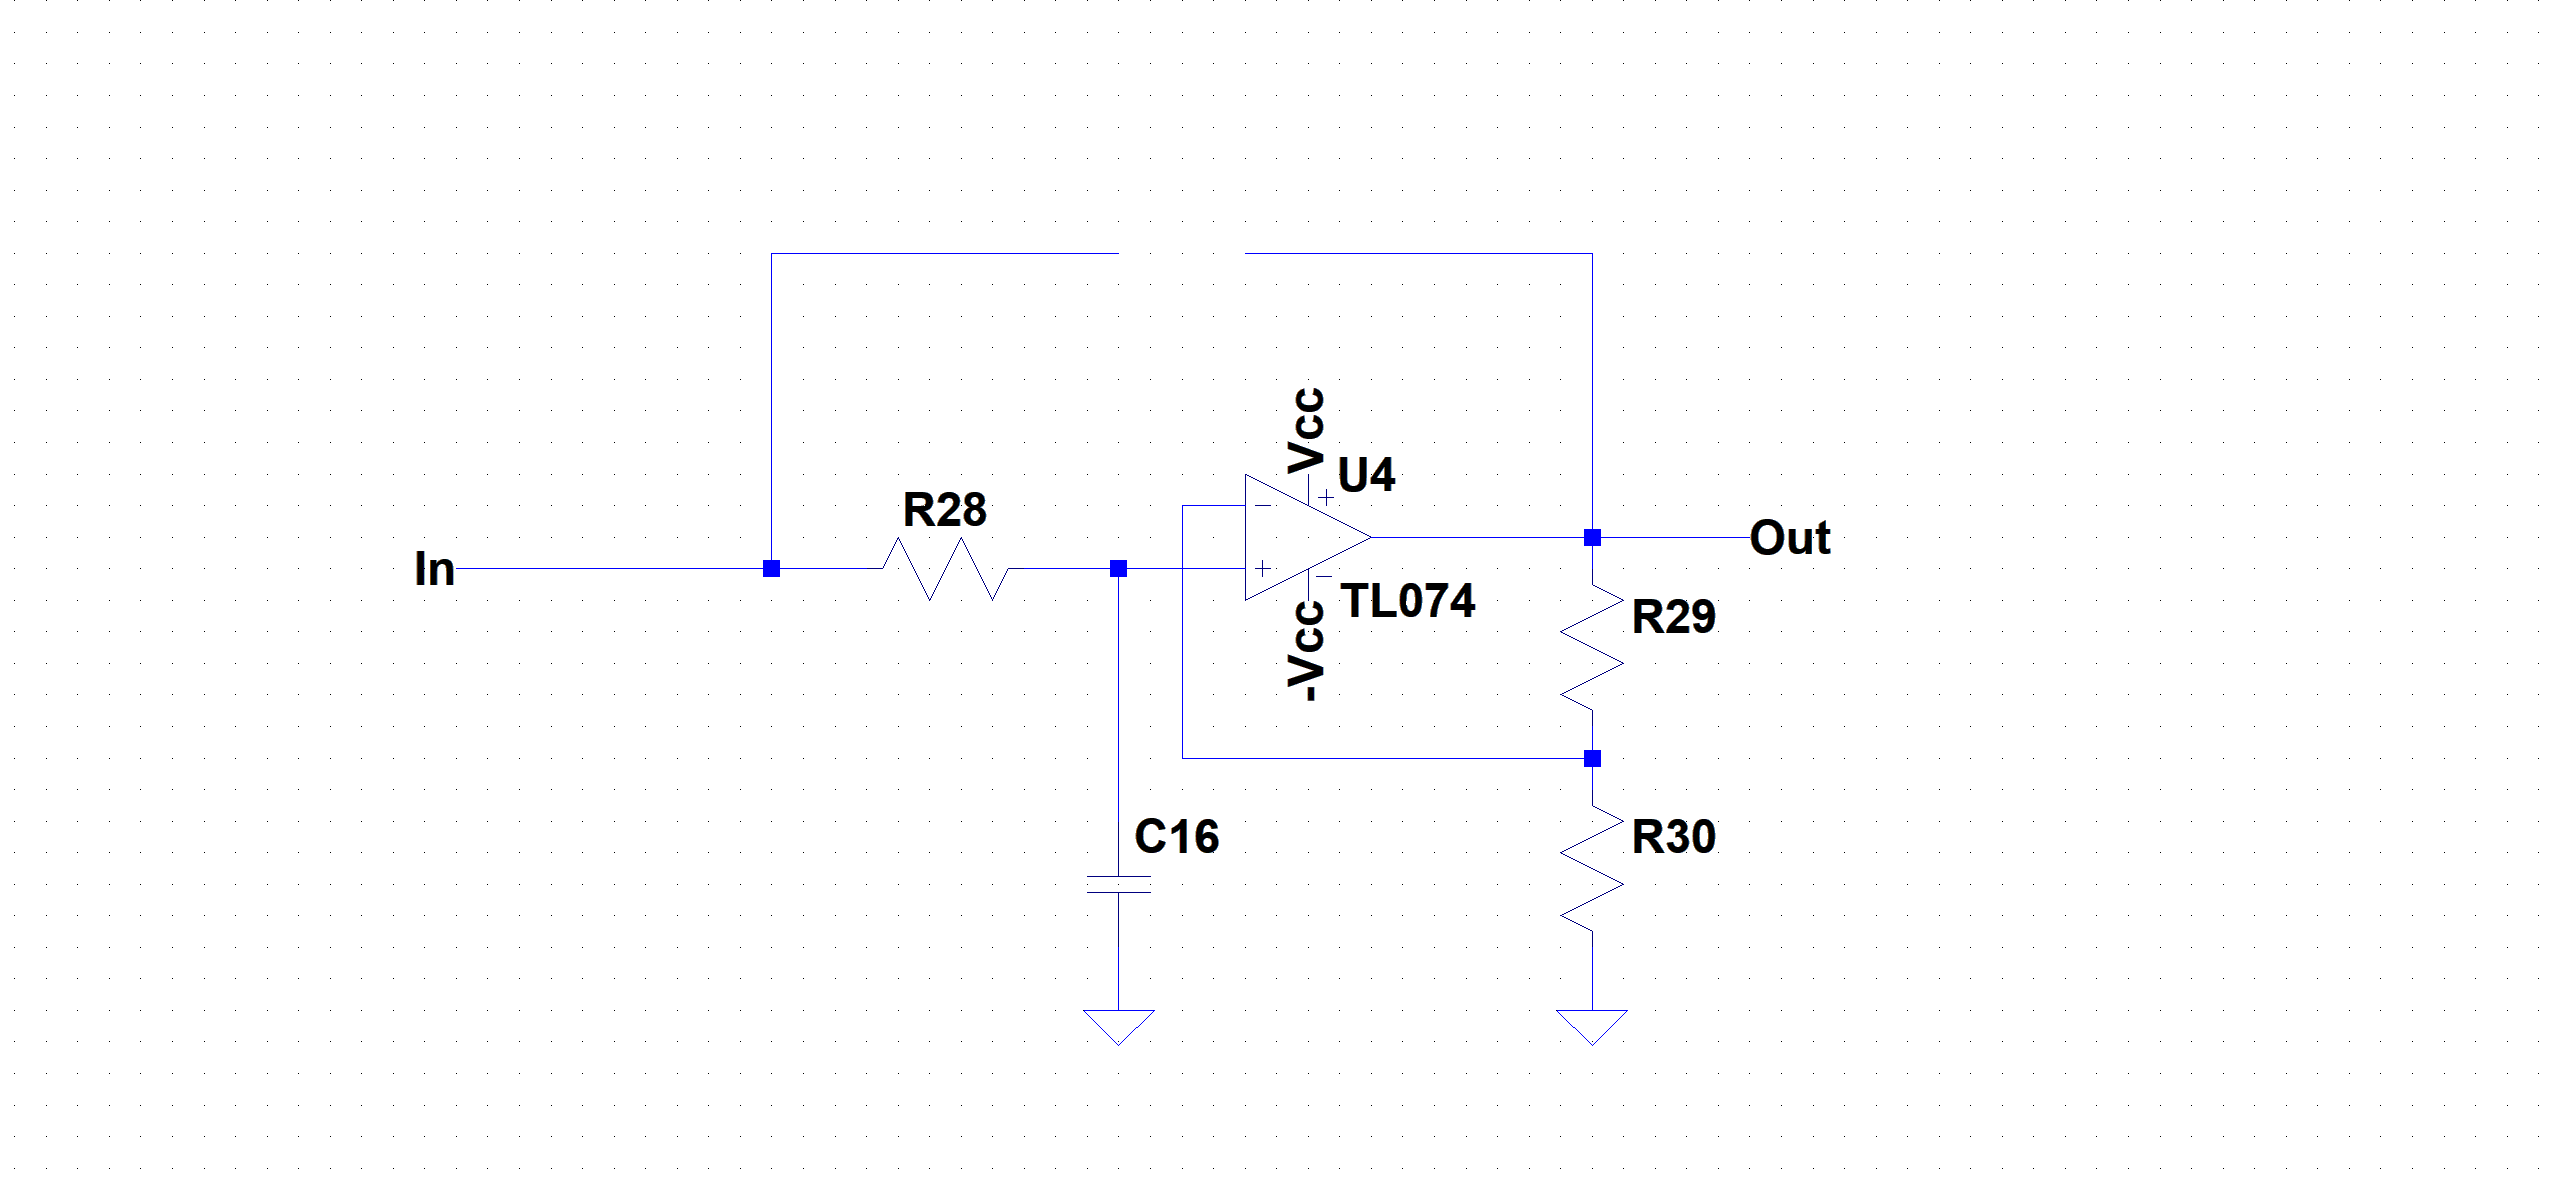
\includegraphics[width=0.9\textwidth]{images/Analoge_Schaltung_Sallentopassive.png}
\caption{Umgebautes Sallen/Key zu passivem Filter 1. Ordnung}
\end{center}
\end{figure}
\end{minipage}

Die Dimensionierung der neuen Schaltung ist mithilfe der nachfolgenden Formel geschehen. Die Verstärkungen konnten beibehalten werden. Die passiven Filter mussten neu berechnet werden.[x]

\begin{minipage}[h]{0.5\textwidth}
\begin{equation}
f_g=\frac{1}{2 \cdot \pi \cdot R_{28} \cdot C_{16}}
\label{eq:Grenzfrequenz}
\end{equation}

\end{minipage}
\begin{minipage}[h]{0.5\textwidth} 
\begin{equation}
A=1+\frac{R_{29}}{R_{30}}
\label{eq:Verstärkung}
\end{equation}
\end{minipage}

%%%%%%%%%%%%%%%%%%%%%%%%%%%%%%%%%%%%%%%%%%%%%%%%%%%%%%%%%%%%%%%%%%%%%%%%%%%
\subsection{Einkoppelung}
Das Signal nach der Filterung und der Verstärkung beträgt $\pm 2.5V$. Um dieses Signal anzuheben auf eine für den Mikrocontroller verträgliche grösse wird eine DC-Spannung eingekoppelt. Nach der Einkoppelung von $2.5V$ bewegt sich das Signal innerhalb von $0V$ bis $5V$. Dies wurde mit folgender Schaltung realisiert.

\begin{minipage}[h]{0.5\textwidth}
\begin{figure}[H]
\begin{center}
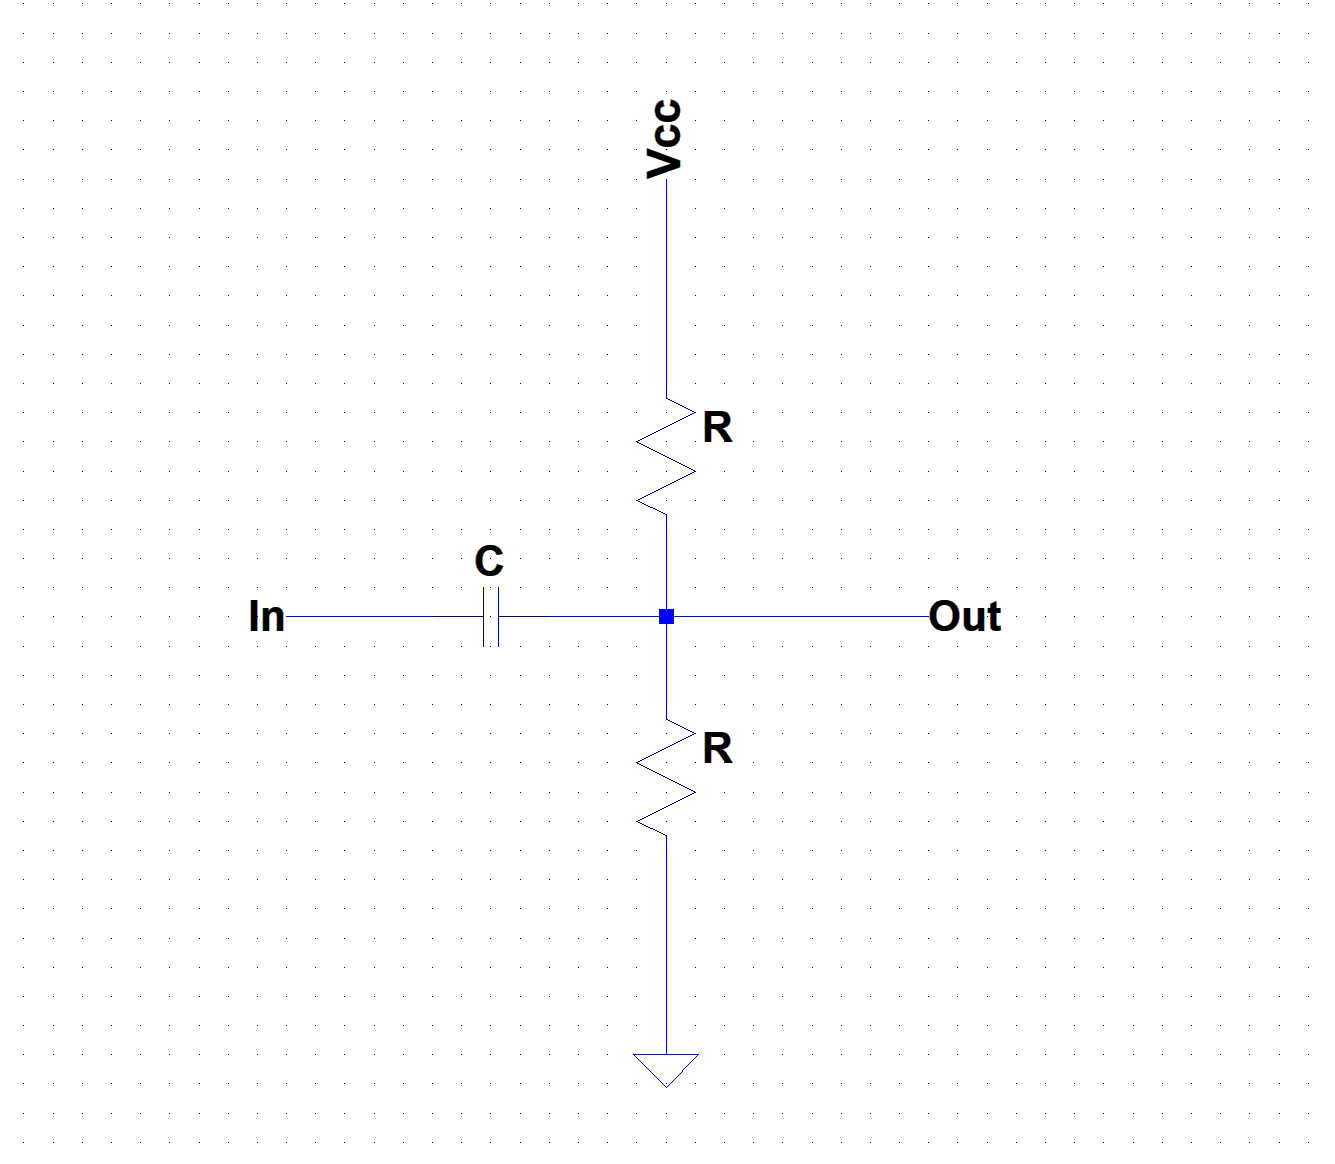
\includegraphics[width=0.9\textwidth]{images/Analoge_Schaltung_Einkoppelung.png}
\caption{Einkoppelung}
\end{center}
\end{figure}
\end{minipage}
\begin{minipage}[h]{0.5\textwidth} 
Um diese Schaltung zu dimensionieren, muss sie auf zwei Arten betrachtet werden. 
Für die AC-Betrachtung ist sie ein Hochpassfilter 1. Ordnung. Dieses Hochpassfilter soll alle Frequenzen passieren lassen ausser Gleichstrom. Für die Dimensionierung kann dieselbe Formel \eqref{eq:Grenzfrequenz} wie für die Tiefpass-Filter verwendet werden. Jedoch wird die Grenzfrequenz $f_g$ auf $0.5 Hz$ gesetzt. $R_{28}$ setzt sich aus den  zwei parallel gesetzten Widerständen zusammen.
\end{minipage}
Für die DC-Betrachtung entspricht die Schaltung einem Spannungsteiler. Der Kondensator stellt in dieser Betrachtung einen Unterbruch dar. Die Widerstände sollten gross gewählt werden, damit die Verluste klein bleiben. Gleichzeitig muss mit den Anforderungen des Hochpassfilters einen Kompromiss gefunden werden. Für unser Projekt war schlussendlich die Grösse des Kondensators ausschlaggebend. Der grösste Kondensator an Lager wurde verwendet.

%%%%%%%%%%%%%%%%%%%%%%%%%%%%%%%%%%%%%%%%%%%%%%%%%%%%%%%%%%%%%%%%%%%%%%%%%%%
\subsection{Sicherheitsschaltung}
\begin{minipage}[h]{0.5\textwidth} 
Um die Eingänge des Mikrocontroller zu schützen wurde eine Sicherheitsschaltung realisiert. Diese schützt den Eingang vor Überspannungen und Unterspannungen. Die obere Diode schaltet, sobald das Eingangssignal oberhalb von Vcc plus der Forward-Voltage der Diode ist. In diesem Fall entsteht ein Kurzschluss zwischen GND und Vcc durch den Operationsverstärker. Um den Strom zu begrenzen ist der Widerstand vorhanden. Gleichzeitig bildet der Widerstand mit dem Kondensator zusammen ein weiteres Tiefpass-Filter, welches hochfrequente Störungen abhalten soll.  Die Grenzfrequenz dieses Filters muss höher sein, als die Grenzfrequenz des ersten Filters, damit es nicht das Signal verfälscht.
\end{minipage}
\begin{minipage}[h]{0.5\textwidth} 
\begin{figure}[H]
\begin{center}
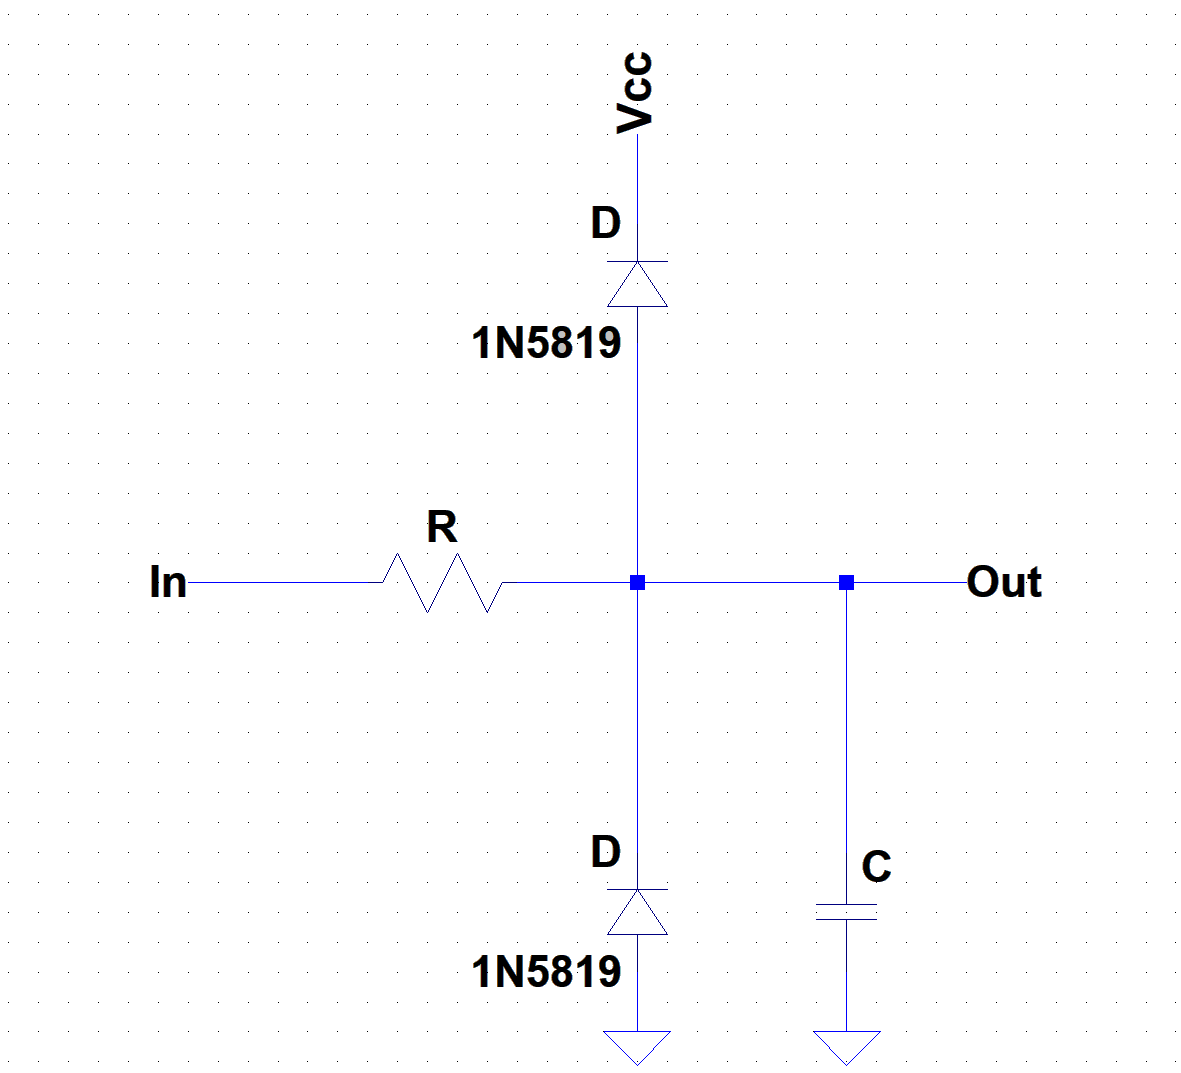
\includegraphics[width=0.9\textwidth]{images/Analoge_Schaltung_Sicherung.png}
\caption{Sicherheitsschaltung}
\end{center}
\end{figure}
\end{minipage}

%%%%%%%%%%%%%%%%%%%%%%%%%%%%%%%%%%%%%%%%%%%%%%%%%%%%%%%%%%%%%%%%%%%%%%%%%%%
\subsection{Genauigkeit}%Marc 1 Seite
%%%%%%%%%%%%%%%%%%%%%%%%%%%%%%%%%%%%%%%%%%%%%%%%%%%%%%%%%%%%%%%%%%%%%%%%%%%
Die Genauigkeit im analogen Schaltungsteil hängt zum einen von den Toleranzen und Ungenaugikeiten der verwendeten Bauteile und zum anderen von der Auflösung des ADCs ab, welcher die Grenze zwischen analog und digital bildet. Die nachfolgende Grafik zeigt den Messpfad mit den möglichen Teilen, in welchen Ungenauigkeiten entstehen können und werden.

\begin{figure}[htb]

	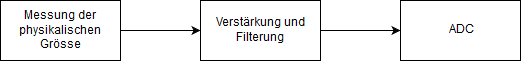
\includegraphics[width=160mm]{images/genauigkeit.png}

	\caption{Messpfad} %picture caption
  
	\label{fig:genauigkeit}

\end{figure}

Nachfolgend werden die möglichen Fehler der einzelnen Blöcke in Abbildung \ref{fig:genauigkeit} erläutert.

\subsubsection*{Messung der physikalischen Grösse}
Der Strom und die Spannung werden jeweils als Spannung über einen bestimmten Widerstand gemessen.Wie aus dem Schema im Anhang unter \textbf{!Noch einfügen!!!} ersichtlich, lässt sich der Strom über das Ohmschen Gesetz $I = \frac{U_{mess}}{R_{mess}}$ berechenen und die Spannung über einen Spannungsteiler $U = U_{mess} \cdot \frac{R_{tot}}{R_{mess}}$. Somit ergeben die Toleranzen der Widerstände eine konstante faktorielle Ungenauigkeiten, welche durch eine Multiplikation im Mikrocontroller beheben wird.

\subsubsection*{Verstärkung und Filterung}
\textbf{!!!!Noch schreiben!!!}

\subsubsection*{ADC}
Bei der Konvertierung eines analogen Signals zu einem Digitalem gibt es zwangsläufig einen Informationsverlust durch die Quantisierung des Signals. Da für dieses Gerät ein 10Bit-ADC verwendet wird, hat das digitale Signal eine Auflösung von 1024 Werten. Für eine Spannung von $\pm$333V bedeutet dies eine Auflösung von 0.65V. Für den Strom ergeben sich folgende Ungenauigkeiten: Der $\pm 15$A Messbereich, ergibt eine Genauigkeit von 19.5mA, der $\pm$5A Bereich, eine von 9.77mA und der Bereich von $\pm$1A, eine Genauigkeit von 1.95mA.

\subsubsection*{Resultierende Genauigkeit} 
\textbf{!!Noch schreiben!!!!}






\pagebreak